\documentclass[tikz,border=10pt]{standalone}
% No extra TikZ libraries needed: all coordinates are explicit.
\begin{document}
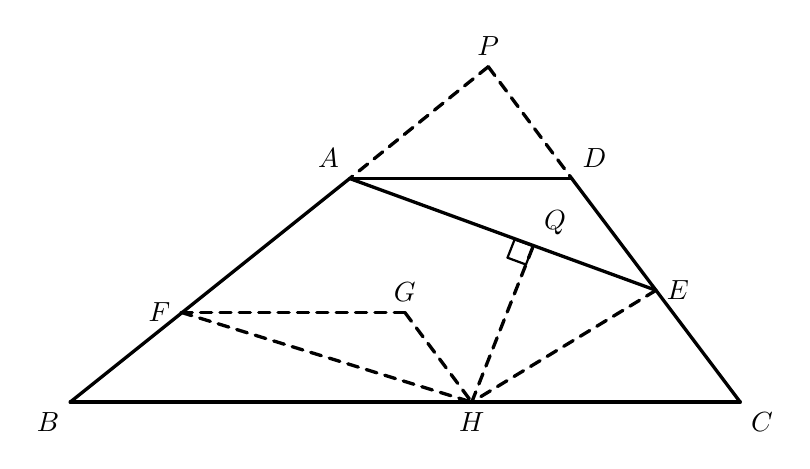
\begin{tikzpicture}[line width=1.2pt, line join=round, line cap=round,
  dsh/.style={dash pattern=on 4pt off 3pt}]

% Named points (x = px/100, y = -py/100)
\coordinate (B) at (1.18,-5.38);
\coordinate (C) at (9.69,-5.38);
\coordinate (H) at (6.28,-5.38);
\coordinate (A) at (4.73,-2.54);
\coordinate (D) at (7.55,-2.54);
\coordinate (P) at (6.49,-1.12);
\coordinate (E) at (8.62,-3.96);
\coordinate (F) at (2.59,-4.24);
\coordinate (G) at (5.43,-4.24);
\coordinate (Q) at (7.06,-3.40);

% Solid segments
\draw (B) -- (C);
\draw (B) -- (A);
\draw (C) -- (D);
\draw (A) -- (D);
\draw (A) -- (E);

% Dashed segments
\draw[dsh] (P) -- (A);
\draw[dsh] (P) -- (D);
\draw[dsh] (F) -- (G);
\draw[dsh] (G) -- (H);
\draw[dsh] (F) -- (H);
\draw[dsh] (E) -- (H);
\draw[dsh] (H) -- (Q);

% Right-angle square at Q between QH and QA (sides along -u_AE and -v_HQ, size 0.25)
\draw[line width=0.8pt] (7.06,-3.40) -- (6.825,-3.314) -- (6.734,-3.546) -- (6.9685,-3.6325) -- cycle;

% Labels
\node[above left] at (A) {$A$};
\node[above right] at (D) {$D$};
\node[above] at (P) {$P$};
\node[above right] at (Q) {$Q$};
\node[left] at (F) {$F$};
\node[above] at (G) {$G$};
\node[right] at (E) {$E$};
\node[below] at (H) {$H$};
\node[below left] at (B) {$B$};
\node[below right] at (C) {$C$};
\end{tikzpicture}
\end{document}